 
%\documentclass[review]{elsarticle}
\documentclass[final,twocolumn]{elsarticle}
%\documentclass[final,5p,times,twocolumn]{elsarticle}
\usepackage{xspace}
\usepackage{project}

%! Author = sbbfti
%! Date = 10/06/2020

\newacronym{ADF}{ADF test}{Augmented Dickey-Fuller test}
\newacronym{KPSS}{KPSS test}{Kwiatkowski-Phillips-Schmidt-Shin test}
\newacronym{ACF}{ACF}{AutoCorrelation function}
\newacronym{PACF}{PACF}{Partial AutoCorrelation function}


\newacronym{ti}{$T_{i}$}{indoor air temperature, $^{\circ}$C}


\begin{document}

    \begin{frontmatter}
%EE6563 Project Progress\\ 
\title{\Huge EE6563 - Final Report\\Footprint Recognition based on \\ Time-Series Classification }
%%$$\title{\Huge CS6735 Research Project \\Footprint Recognition based on \\ Time-series classification }

%% Group authors per affiliation:
\author{Saeed Kazemi\fnref{myfootnote}}
%%$$\author{Maryam Sepasi\fnref{myfootnote1}}
\address{University of New Brunswick}
\fntext[myfootnote]{Saeed.Kazemi@unb.ca.}
%%$$\fntext[myfootnote1]{maryam.sepasi@unb.ca.}

%% or include affiliations in footnotes:
%\ead[url]{https://github.com/SKazemii/EE6563}

\begin{abstract}
Given present-day security concerns, many buildings have implemented robust authentication techniques. Aside from authentication to enter a building, applications such as border and airport security also administer identification. Therefore, many cities and companies provide technologies like CCTV or fingerprinting for authentication and verification. But each system has its own drawbacks. For example, due to the Covid-19 pandemic, most people wear a mask and avoid touching unnecessary surfaces. Thus, gait recognition could be a solution. 



%In this project, we worked on temporal information of time-series data. These features used to construct a classifier. Moreover, verification mode was used for this research.

%This aids to disguise people and reduces the hygiene of fingerprint biometrics respectively. In this research, we focus on which classifier has better results on barefoot footprints and which features have the important effect on the classifier.


%%$$In this paper, we present a review of the time series approaches for classification tasks including conventional machine learning algorithms and Deep Neural Networks. Also, in \ref{appendix:2}, more approaches have been reviewed for time series classification. These approaches were implemented in verification mode. Experimental results show that the SVM classifier on the contribution of all handcrafted features had the best performance with 91.3\%.

In this paper, we present a review of the time series approaches for classification tasks including conventional machine learning algorithms and Deep Neural Networks. These approaches were implemented in verification mode. Experimental results show that the SVM classifier on the contribution of all handcrafted features had the best performance with 91.3\%.

%Convolutional Neural Networks (CNN) has achieved a great success in image recognition task by automaticallylearning a hierarchical feature representation from raw data. While the majority of Time-Series Classification(TSC) literature is focused on 1D signals, this paper uses Recurrence Plots (RP) to transform time-series into2D texture images and then take advantage of the deep CNN classifier.  Image representation of time-seriesintroduces different feature types that are not available for 1D signals, and therefore TSC can be treated astexture image recognition task. CNN model also allows learning different levels of representations together witha classifier, jointly and automatically. Therefore, using RP and CNN ina unified framework is expected to boostthe recognition rate of TSC. Experimental results on the UCR time-series classification archive demonstratecompetitive accuracy of the proposed approach, compared not only to the existing deep architectures, but alsoto the state-of-the art TSC algorithms.


\end{abstract}

\begin{keyword}
Footprint recognition\sep Time-series classification\sep pressure sensor
\end{keyword}

\end{frontmatter}


    \section{Introduction}

Contemporary security identification has led to a plethora of biometric-based authentication systems. From palm readers at testing centers to facial recognition on smartphones, many systems are now used to regularly verify identities. These inherence-based systems are attractive in comparison to knowledge or possession-based methods of authentication because biometrics are unique, unforgettable, and far more difficult to steal than a password or swipe card.

Although biometric identification appears sophisticated when compared to something like physical keys, it does not come without its own share of caveats. For example, owing to the ongoing Covid19 pandemic, many people wear masks when outside of their house, challenging most facial recognition systems. Additionally, biometrics that rely on touch, such as fingerprinting, raise safety concerns, as the scanner may become a vector for virus transmission. Despite these setbacks, given their merits and widespread deployment, biometric identification systems are unlikely to disappear.

One behavioral biometric that has gained recent success and is worth further consideration given current constraints is gait recognition. Usage of gait recognition has grown in the security industry in recent decades due to advances in deep learning. Singh et al. \cite{Singh2019APerspectives} categorized gait recognition into two main categories, vision-based and sensor-based. In vision-based approaches, cameras capture data of a person walking for the purpose of gait recognition. Sensor-based gait recognition is performed using either wearable sensors which produce kinematic data, or floor sensors which produce kinetic data \cite{Connor2018BiometricFeatures}.

%\section{Datasets}
This paper focused on analysing kinetic data. For this purpose, the Stepscan dataset which is a private dataset was used \cite{Connor2015ComparingBiometrics}. This dataset was obtained from high-resolution floor tiles that have recently been introduced by Stepscan Technologies Inc. Furthermore, this dataset consists of a spatial-temporal tensor, X, with dimensions $S \times T \times H \times W$ where $S$ represents the number of samples. $T$ is the number of temporal observations or video frames; $H$ and $W$ are the dimension of the image in pixels. Figure \ref{fig:Stepscan_dataset} indicates three frames from one of samples in the dataset.  

\begin{figure}
    \centering
    \begin{minipage}[b]{.5\textwidth}
        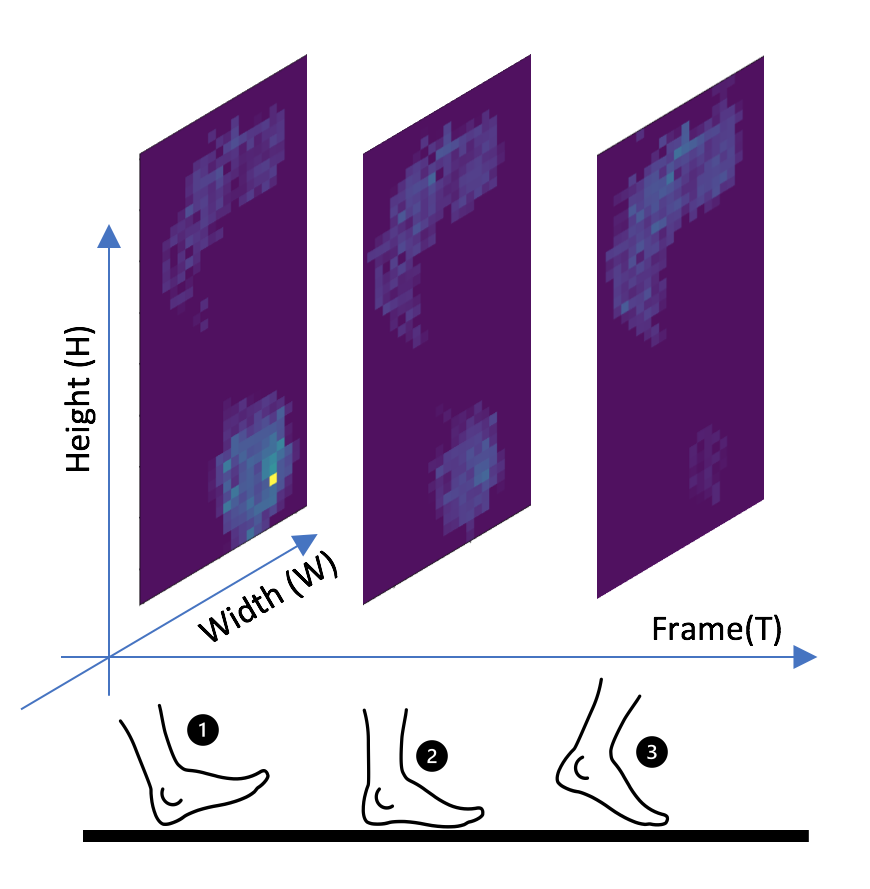
\includegraphics[width=\textwidth]{figures/project/frame2.png}
    \end{minipage}
    \caption{Different frames of footprint video in Stepscan dataset.}
    \label{fig:Stepscan_dataset}
\end{figure}

%%************
In general, there are two modes for footprint recognition or generally in the biometric system: verification or identification mode \cite{Jain2004AnRecognition}. In verification mode, the biometric system is used for accessing buildings or data. In other words, the system compares the claimed person with its dataset to determine whether or not the claim is valid. These systems not only consume less processing power and time but also have better performance regarding identification systems \cite{Jain2004AnRecognition}. Moreover, verification systems could be implemented on a small scale. This project aims to find some features from the datasets to construct a classifier for verification purposes. 

%Because verification systems only need to compare the presented biometric to a biometric reference stored in the system, they can generate results more quickly and are more accurate than identification systems, even when the size of the database increases.


The rest of this paper is organized as follows: Section 2 provides the relevant works and researches. Then, the classification method based on machine learning and deep learning is presented in Section 3. The results and discussion are described in Sections 4 and 5.

%%$$The rest of this paper is organized as follows: Section 2 provides the relevant works and researches. Then, the classification method based on machine learning and deep learning is presented in Section 3. Also a brief survey on time series classification and Deep learning is provided in \ref{appendix:2}. The results and discussion are described in Sections 4 and 5.

% in Section 3, the time domain features as well as machine learning models are defined. In Section 4, we discuss the results, and we propose future work in Section 5.



Furthermore, this research will be implemented in Python, and the source codes are available on the GitHub repository \cite{SKazemii/EE6563}. 











    \section{Literature Review}

%\subsection{The subsection also appears in the bookmarks}
DARPA, the Defense Advanced Research Projects Agency of the USA, started to research gait recognition by vision data in the early 2000s \cite{Connor2018BiometricFeatures}. Besides vision data \cite{Chen2006GaitModel}, some studies have instead used accelerometry from smartphones \cite{Mantyjarvi2005IdentifyingAccelerometers}, audio \cite{Geiger2013Gait-basedFeatures}, and underfoot pressures data \cite{Nakajima2000Footprint-BasedRecognition}. 

Addlesee in \cite{Addlesee1997TheFloor} used a new sensor (Active floor) for the first investigations into footprint recognition. This sensor was a square carpet tile maintained at the corners by some load cells and supplied the \gls{grf}. Orr and Abowd \cite{Orr2000TheTracking} extracted ten temporal features from the \gls{grf} curve. 

Moustakidis et al. \cite{Moustakidis2008SubjectSignals} extracted temporal features from the wavelet decomposition of \gls{grf} and then applied a kernel-based support vector machine. These studies have limitations in terms of the small sample sizes used for classification (e.g., 15 \cite{Orr2000TheTracking}, 10 \cite{Moustakidis2008SubjectSignals}, and 15 \cite{MiddletonARecognition}), and moderate classification rates ($CR < 90\%$).

Pataky in \cite{Pataky2012GaitIndividuals} achieved a 99.6\% classification rate in a 104-participant dataset. This result was based on spatial alignment and automated dimensionality reduction. He used a template image that was made in \cite{Pataky2011AnEvaluation}. Pataky named this template the Munster-104 template.

In 2015, Cantoral-Ceballos \cite{Cantoral-Ceballos2015IntelligentEnvironments} introduced an intelligent carpet system. This carpet system (iMAGiMAT) worked based on the deformation of 116 distributed \gls{pof}. So that applying pressure to this system would change the intensity of the transmitted light. Thus the nature of the output of this sensor is time-series data.
 
Costilla-Reyes et al. \cite{Costilla-Reyes2016TemporalSystem} extracted five features directly from raw data of the iMAGiMAT sensor. These features were spatial Average (SA), standard deviation (SD), adjacent mean (AM), cumulative sum (CS), and cumulative product (CP).
They implemented 14 various machine learning methods for classification. The best result belonged to the Random Forest model with a validation score of $90.84 \pm 2.46\%$. 

 
%**Almost all machine learning approaches, except for those based on deep learning, require feature extracting process. These process can cause some information to be loss by expert mistake. On the contrary, deep learning models already incorporate this kind of feature engineering internally, optimizing it and eliminating the need to do it manually. Therefore they are able to extract information from the time series in a faster, more direct, and more complete way.
Costilla-Reyes et al. in \cite{Costilla-Reyes2018DeepSensors} used an end-to-end convolutional neural network to extract Spatio-temporal features automatically. This technique increased F-score performance to about 97.88\% $\pm$ 1.7\%. They reconstructed pressure images from the time-series data to feed to deep networks. Some papers used other techniques like Continuous Wavelet Transform (CWT) \cite{Wang2021AutomaticNetwork}, Recurrence Plots (RP) \cite{Hatami2017ClassificationNetworks}, and short-time Fourier transform (STFT) \cite{Huang2019ECGNetwork} to produce a 2D representation of time-series. Therefore, time series classification can change to a texture image recognition task.


 

%Barandas et al. in \cite{Barandas2020TSFEL:Library} introduced a Python package entitled Time Series Feature Extraction Library (TSFEL). This Python package could compute more than 60 different features from the time-series data.


% The UoM-Gait-Dataset was obtained from iMAGiMAT sensor \cite{Cantoral-Ceballos2015IntelligentEnvironments} (an optical floor sensor). This sensor contains about 160 distributed \gls{pof} that indicate the foot pressure signals over time. Some studies like \cite{Costilla-Reyes2020DeepHealthcare} used this dataset to construct images for their research.

    \input{manuscript/src/Questions/B3-Methodology}

    %\section{Constraints}
%The constraints in this project could fall into two groups. The first constraint is related to the limitation on laboratory conditions \cite{Connor2018BiometricFeatures}. In real-world circumstances, many situations such as walking speed, clothing, footwear, and load carriage could affect our results, whereas our datasets could cover some of these real-world conditions. For example, except for the walking speed and footwear, both datasets do not have useful information for other real-world situations. Consequently, our results are optimistically biased. Table \ref{tab:1_vul} indicates some inhibiting factors. 

%Another significant limitation in the Stepscan dataset is the lack of relative footprint location. The dataset included only aligned and segmented footprint images. The location of samples concerning each other is unknown. This information could play a significant role in predicting the location of future footsteps. 

%\begin{center}
%	\begin{table}[!t]
%	\caption{Some inhibiting factors in gait recognition.}
%	\label{tab:1_vul}
%	\hspace{3em}
%	\setlength\extrarowheight{-2pt}
%	\begin{tabular}{rl}
\toprule
    &  Inhibit Factors \\
\midrule
  1 & Footwear               \\
  2 & clothing               \\
  3 & Injury                 \\
  4 & Muscle development     \\
  5 & Fatigue                \\
  6 & Age                    \\
  7 & Load carriage          \\
  8 & Walking speed          \\
  
\bottomrule
\end{tabular}


%	\end{table}
%\end{center}
 

%\section{Remaining Work}

%In recent years, improvements in the computational process of computers and other benefits of \gls{dnn} have caused many researchers (like \cite{IsmailFawaz2019DeepReview} and \cite{Costilla-Reyes2018DeepSensors}) to move towards \gls{dnn} for the classification of time series data. Therefore, these algorithms will be reviewed in a later stage of this project.

%Because the entire time series were considered for extracting features, we have had one value for each attribute. For instance, while local maximums could be good features, the algorithm returned only the global maximum as a Max feature. We could slide a window on the signal to extract handcrafted features. It causes only a part of the data to consider in each moment. In other words, because each data includes several stages of the walking cycle, features should be extracted according to these periods.   

%Moreover, cropping the heel or toe area in each video could separate features based on the walking stages (pressure area). By this means, each video will be divided into N sub-area, and then for each region, we reconstruct time-series signals and extract features. As a result, these features belong only to that area or stage of walking.

%Due to using the aligned video, we could consider some pixels over time as 2D signals. Although our features space increased rapidly, we could put a threshold on variance and energy of time-series signals for controlling features space. 

%In this research, regardless of eliminating high-correlated and low variance features, we should use a more complex feature selection algorithm to eliminated irrelevant and redundant ones. This reduction might increase the accuracy.

%In addition, it had better to split the dataset into left and right footprints for exploring the effects of extracted features on classifier accuracy. 
 

\section{Experimental Results}
The biometrics industry has utilized two performance measurements, False Rejection Rate (FRR) and False Acceptance Rate (FAR), for accuracy. These measures also are called False Negative Rate (FNR) and False Positive Rate (FPR) in biometric literature. According to these values, a graphical ROC curve was produced by plotting FPR on the x-axis against 1–FNR on the y-axis. Figure \ref{fig:ROC} shows the ROC curves for different models and features. 

The area under the ROC curve (AUC) shows the performance of verification systems. An AUC of 0.5 represents a system with no discriminating ability (The blue line in figure \ref{fig:ROC}), whereas an AUC of 1.0 represents a test with perfect discrimination. Moreover, many researchers often use equal error rate (EER) as an additional metric to describe the performance of biometric systems. EER refers to the point that FRR equals FAR. The smaller value of EER shows the better performance. Results of four different machine learning algorithms in several types of features are shown in table \ref{tab:1_ML}.


For the training scenario, the first 50 users were used for developing models while other users set aside as imposter data. Then for each subject, a binary classifier was trained based on 80 percent data (about 16 in-class samples and 16 $\times$ 49 $\approx$ 780 samples from impostor class). For testing, a set of four genuine samples and 4 $\times$ 49 $\approx$ 190 from impostor samples were used. Due to the fact that we developed a model for each subject, the average of FPR and FNR was calculated for each method.

The SVM classifier’s best AUC was 91.3\%, as shown in table \ref{tab:1_ML}. This result was achieved by classifying the combination of all features and the best AUC among all approaches. Other algorithms had similar performance on all features. All kinds of features had the worst results on Random Forests Classifiers. In terms of the EER metric, the SVM classifier achieved the smallest value (about 0.147) on all handcrafted features.









%The SVM performed best with the mixture of all features, at 56\% accuracy (see table \ref{tab:1_ML}). All other feature subsets achieved lower than this amount. The worst performance for all these classifiers belonged to the random forest classifier with about 30\%.



%The area under the ROC curve (AUC) is a global measure of the ability of a test to discriminate whether a specific condition is present or not present. An AUC of 0.5 represents a test with no discriminating ability (ie, no better than chance), while an AUC of 1.0 represents a test with perfect discrimination. The (unpublished) ROC curve for ACS (figure 1) which was generated from the T-MACS scores calculated for the derivation set has an AUC of 0.94 after correction for in-sample optimism by cross-validation, which would suggest that T-MACS score is a very good discriminator of ACS versus no ACS.


 


\begin{center}
	\begin{table}[!t]
	\centering
	\caption{The EER and AUC metric for Machine learning models implemented in this paper.}
	\label{tab:1_ML}
	%\hspace{-1em}
%	\setlength\extrarowheight{-2pt}
	\begin{tabular}{llll}
\toprule
{} &  Frame Work &    AUC &    EER \\
\midrule
0  &     LDA\_ALL &  0.884 &  0.202 \\
1  &    LDA\_SPEC &   0.87 &  0.193 \\
2  &    LDA\_STAT &  0.877 &  0.206 \\
3  &    LDA\_TEMP &  0.881 &  0.215 \\
4  &     LDA\_VGG &   0.75 &  0.306 \\
5  &  LDA\_MOBNET &  0.766 &  0.298 \\
6  &     KNN\_ALL &  0.841 &  0.202 \\
7  &    KNN\_SPEC &  0.811 &  0.228 \\
8  &    KNN\_STAT &  0.822 &  0.206 \\
9  &    KNN\_TEMP &  0.819 &  0.222 \\
10 &     KNN\_VGG &  0.606 &  0.418 \\
11 &  KNN\_MOBNET &   0.63 &  0.404 \\
12 &     SVM\_ALL &  0.913 &  0.147 \\
13 &    SVM\_SPEC &  0.606 &  0.412 \\
14 &    SVM\_STAT &  0.741 &  0.306 \\
15 &    SVM\_TEMP &  0.883 &  0.203 \\
16 &  SVM\_MOBNET &   0.76 &  0.286 \\
17 &     RFC\_ALL &  0.651 &  0.402 \\
18 &    RFC\_SPEC &  0.598 &  0.441 \\
19 &    RFC\_STAT &  0.565 &  0.465 \\
20 &    RFC\_TEMP &  0.608 &  0.438 \\
21 &     RFC\_VGG &  0.573 &  0.453 \\
22 &  RFC\_MOBNET &  0.586 &  0.452 \\
23 &         FCN &  0.798 &  0.285 \\
\bottomrule
\end{tabular}

	\end{table}
\end{center}

\begin{figure}
     \centering
     \begin{subfigure}[b]{0.45\textwidth}
         \centering
         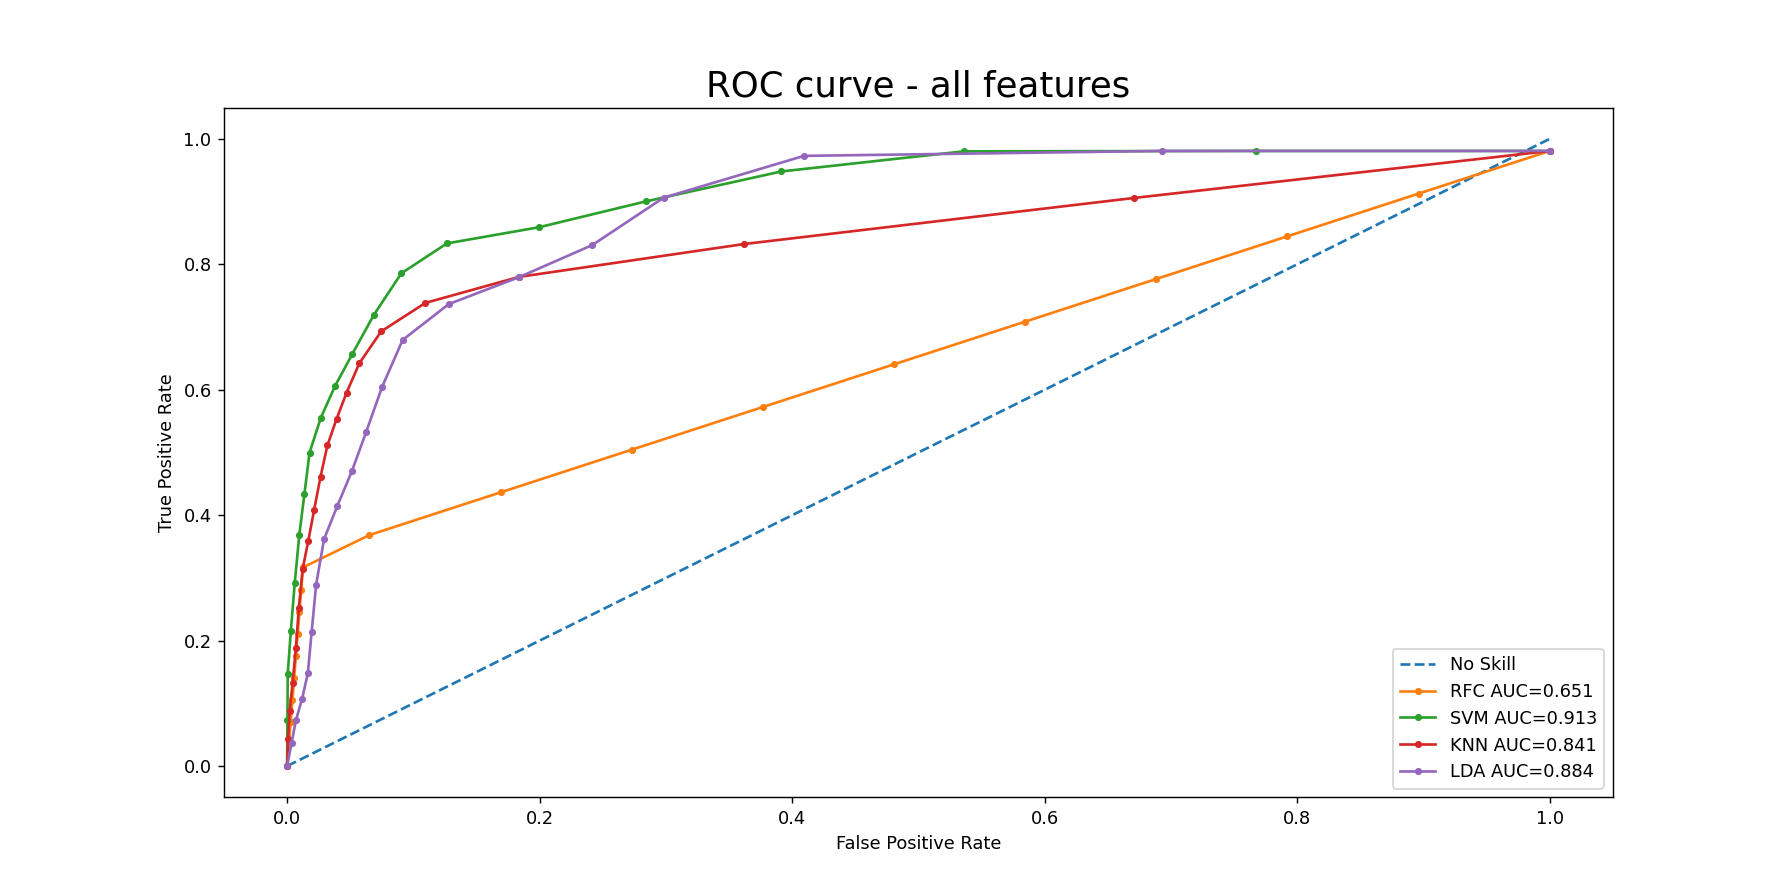
\includegraphics[width=1\textwidth]{manuscript/src/figures/project/roc_curve_all 2021-04-09-11:12:24-tree-Mobnet-standardization.png}
         \caption{The ROC curve of four Machine learning algorithms on handcrafted features}
         \label{fig:ROC_all}
     \end{subfigure}
     \hfill
     \begin{subfigure}[b]{0.45\textwidth}
         \centering
         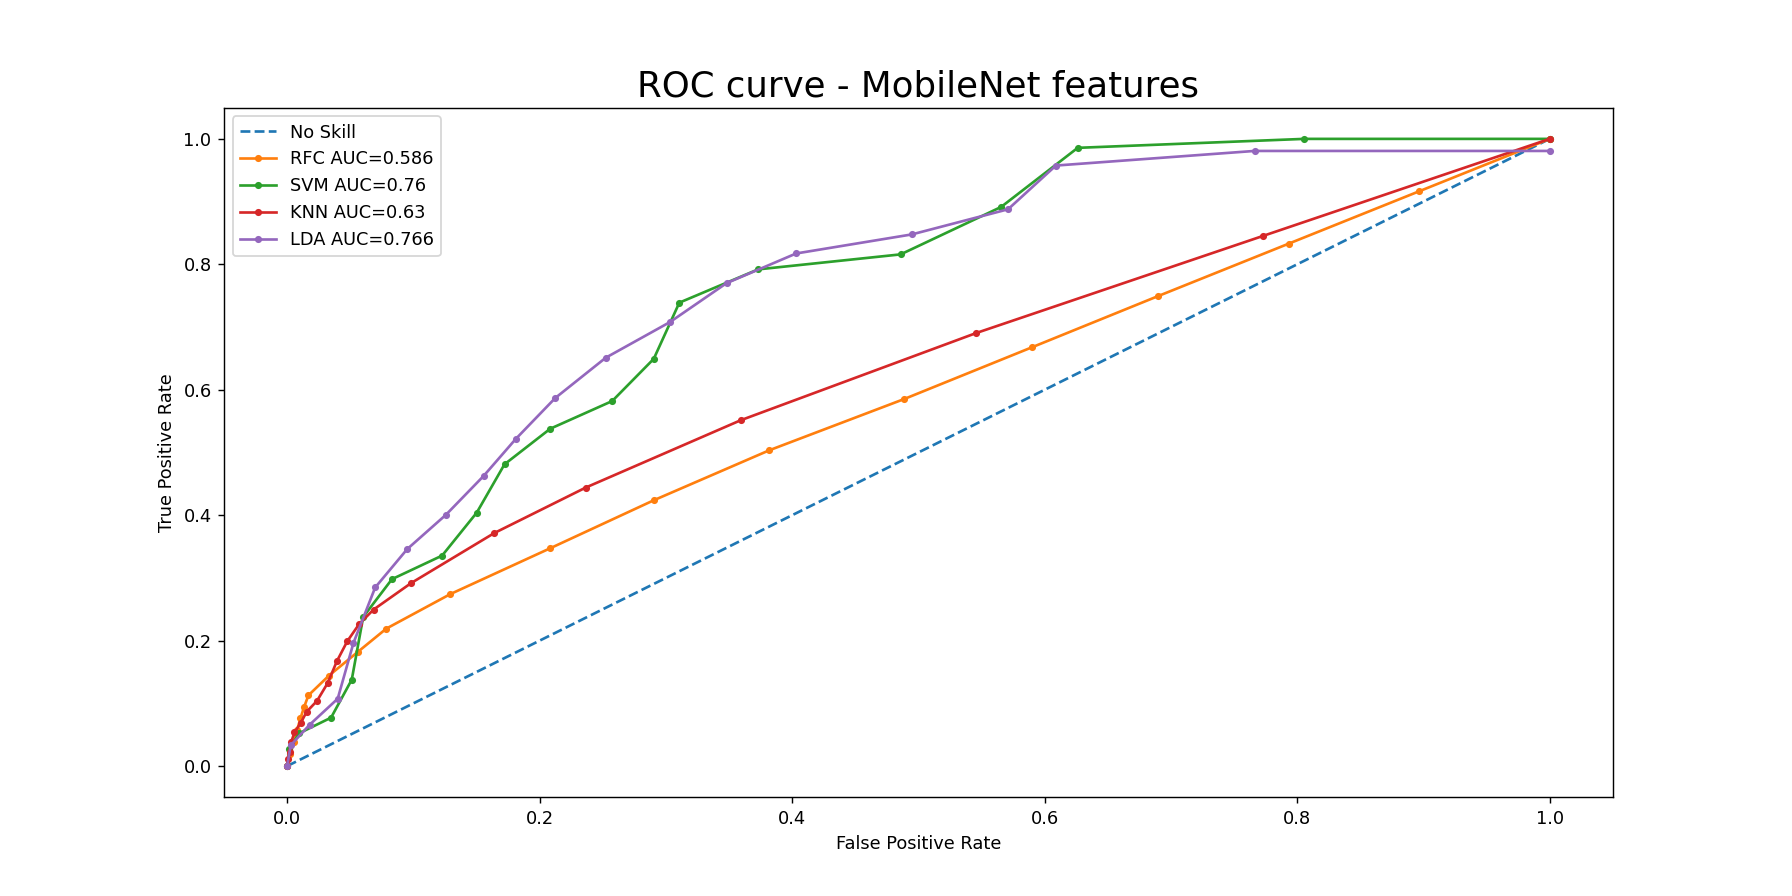
\includegraphics[width=\textwidth]{manuscript/src/figures/project/roc_curve_MobileNet 2021-04-09-11:12:24-tree-Mobnet-standardization.png}
         \caption{The ROC curve of four Machine learning algorithms on MobileNet features}
         \label{fig:ROC_Mob}
     \end{subfigure}
     \vfill
     \begin{subfigure}[b]{0.45\textwidth}
         \centering
         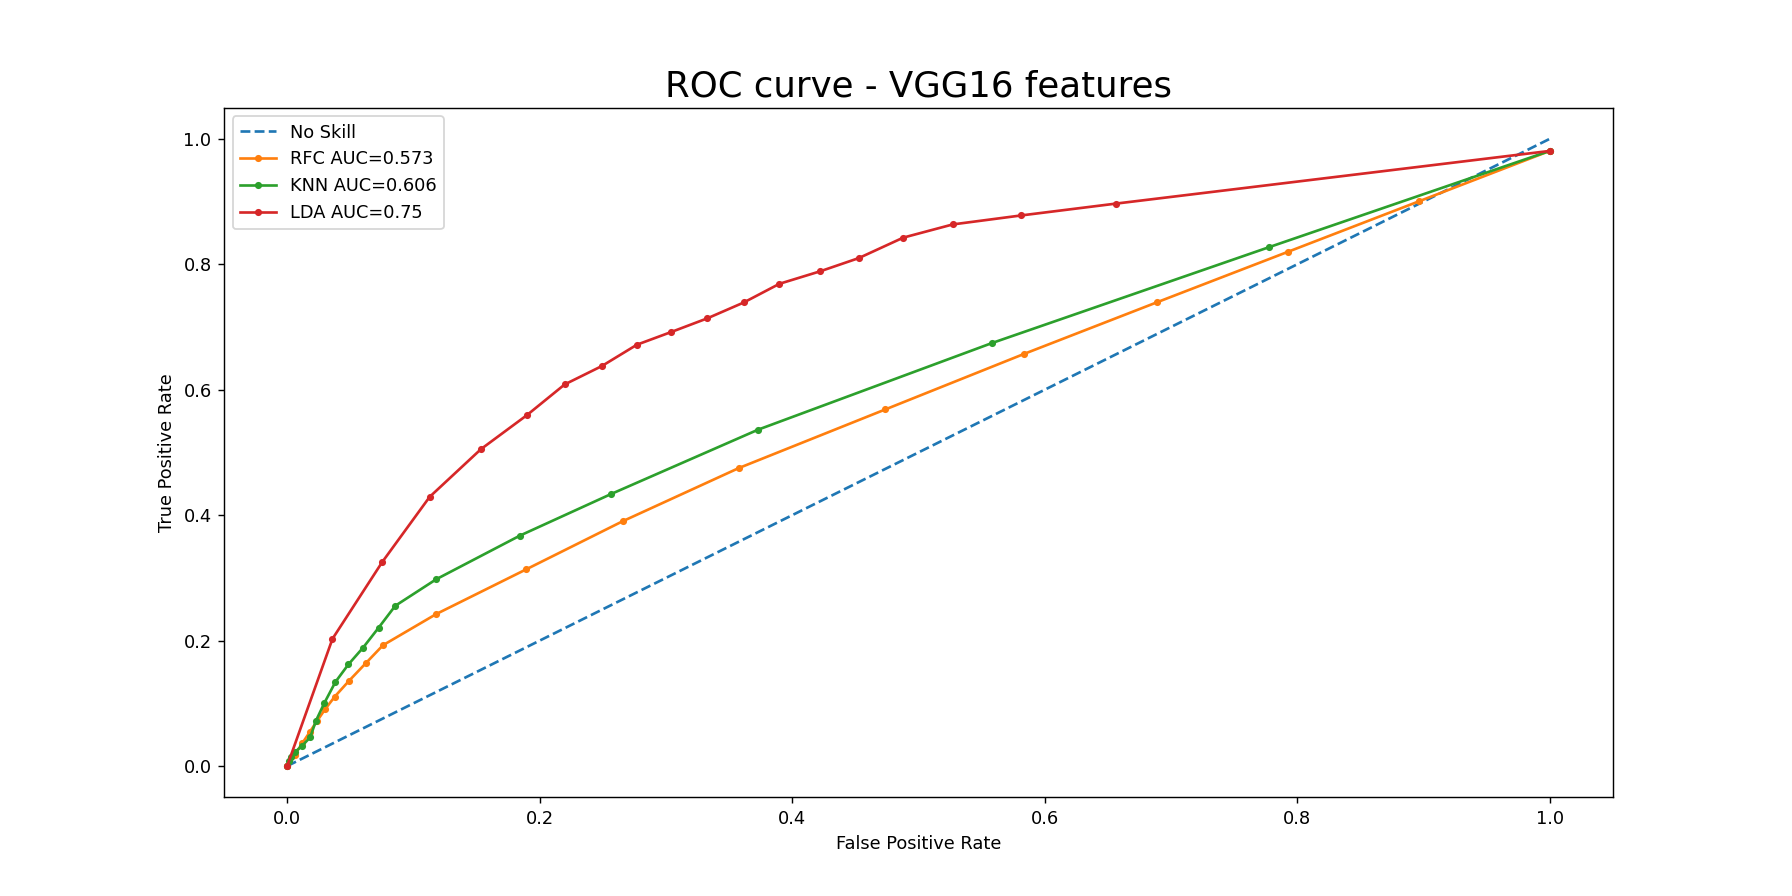
\includegraphics[width=\textwidth]{manuscript/src/figures/project/roc_curve_vgg 2021-04-09-11:12:24-tree-Mobnet-standardization.png}
         \caption{The ROC curve of four Machine learning algorithms on VGG16 features}
         \label{fig:ROC_vgg}
     \end{subfigure}
     \hfill
     \begin{subfigure}[b]{.45\textwidth}
         \centering
         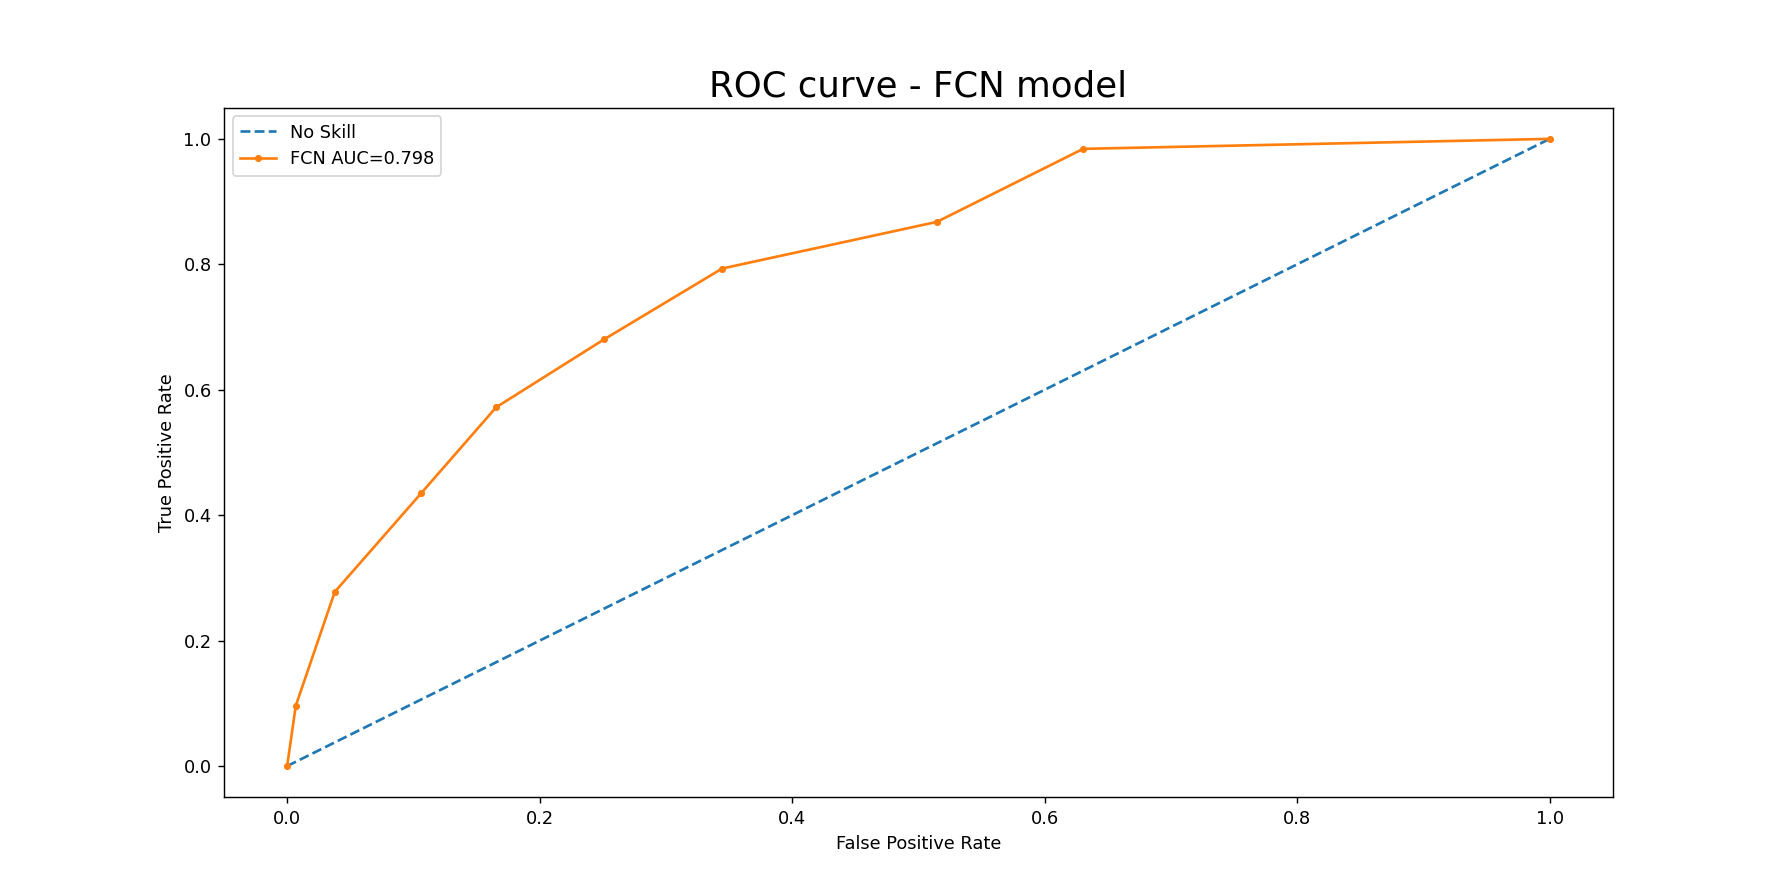
\includegraphics[width=1\textwidth]{manuscript/src/figures/project/roc_curve_FCN 2021-04-09-11:12:24-tree-Mobnet-standardization.png}
         \caption{The ROC curve of Fully Convolutional Network (FCN).}
         \label{fig:ROC_fcn}
     \end{subfigure} 
        \caption{The ROC curve of different approaches}
        \label{fig:ROC}
\end{figure}

%Fig. 9 shows the ROC curves using the test set, indicating that all the hybrid methods achieved higher AUC values than a single conventional classifier. Specifically, the CNN-SVM and CNN-RF methods obtained higher AUC values of 0.868 and 0.829 than SVM and RF, respectively. Furthermore, compared to LR, the CNN-LR method achieved the most significant improvement of 0.063 in terms of AUC. In addition, the AUC value obtained by CNN was higher than single machine learning classifiers, but lower than the hybrid methods. 


    \section{Discussion Progress}
%%%***This is largely a recap of the results, but not much of a discussion about why.  A discussion should careful consider why you got the results you did, and how it relates to what you expected and other works.

The results indicate that spectral features are more powerful features for all machine learning algorithms. The reason behind this might be the number of features and their qualities in this set. Based on table \ref{tab:Features_list}, there are about 300 features for this set, much more than two others.

Another feature that has a significant effect on the accuracy is inter stride distance. This feature has been added only to all features and increased the accuracy of LDA from 60\% to 69\%. 
 
The results might suggest that using AR features are not significant impact on accuracy. The accuracy of LDA without these features reduced to 68.57\%. 

Unbalance dataset also could have negative effect on the results. For example in the Stepscan dataset, there are about 800 negative class whereas 16 samples associated with the positive class. Consequently, the models were biased towards the negative class. 


The poor results of the transfer learning framework might be the fact that only machine learning algorithms were trained based on the Stepscan dataset. It could have better result if we train last two layer of CNNs. 





%The LDA classifier’s best performance was a 69.2\% accuracy, as shown in table \ref{tab:1_ML}. This result comes from classifying the combination of all features. The kNN algorithm had similar performance on all kinds of features except \gls{AR} features. All algorithms had the worst results on this group of features.

%The SVM performed best with the mixture of all features, at 56\% accuracy (see table \ref{tab:1_ML}). All other feature subsets achieved lower than this amount. The worst performance for all these classifiers belonged to the random forest classifier with about 30\%.

%The results do not fit with the theory that…
%The experiment provides a new insight into the relationship between…

%The data contributes a clearer understanding of…
%While previous research has focused on X, these results demonstrate that Y.
%The generalizability of the results is limited by…
%The reliability of this data is impacted by…
%The methodological choices were constrained by…
%It is beyond the scope of this study to…







%    \newpage
%    \section{CNN}



\paragraph{Functionality} The Elsevier article class is based on the standard article class and supports almost all of the functionality of that class. In addition, it features commands and options to format the
\begin{itemize}%\begin{enumerate}[(1)]
\item document style
\item baselineskip
\end{itemize}



\begin{figure}
    \centering
    \begin{minipage}[b]{.5\textwidth}
        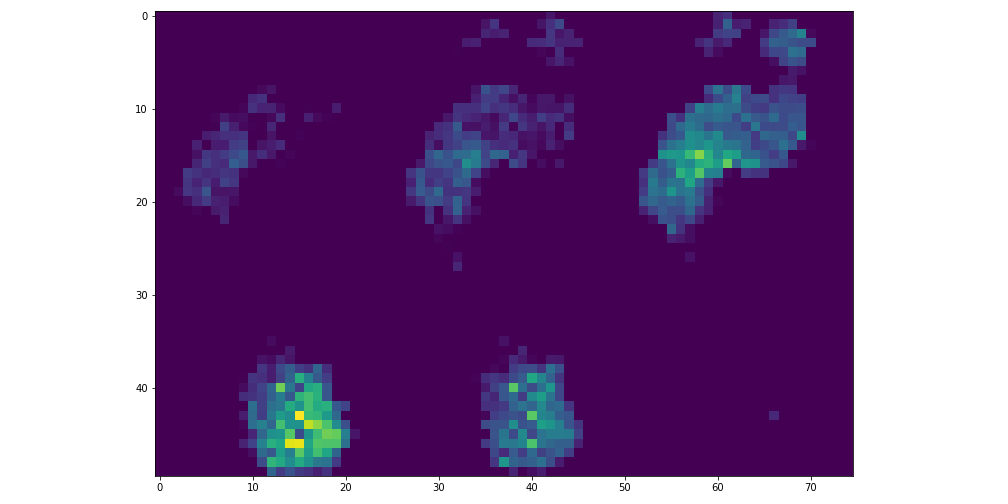
\includegraphics[width=\textwidth]{figures/project/frame1.png}
    \end{minipage}
    \caption{sample image.}
    \label{fig:Stepscan_dataset}
\end{figure}


Here are two sample references: \cite{SKazemii/EE6563}.
    
%\section*{\#TODO:}
%\begin{enumerate}[(1)]
%\item should normalized
%\item You want to focus on temporal information, and how it will help.\\

%\item Aren't they both time-series?  Are you just referring to the method that they are stored?   An array of images over time (video) is still a time series.\\ 
%\item You should show them as separate frames; how can you show the temporal aspects better?\\
%\item But these are just spatial features plotted over time? What are the proposed temporal features? \\
%\item Are you only thinking about within cycle information?  What about inter-stride information?  (for example, inter-stride variability is a well known gait feature).\\
%\item Have you explored relationships between pixels/features over time?
%\item Does Costilla-Reye's work deserve a bit more discussion?  Is that the current state-of-the-art?
 

%\item Focus on what is important; where is the temporal information going to come from?  Time series of spatial information?  Temporal features?  Temporal algorithms applied to spatial features?  Are the features only within stride, or are your features going to be inter-stride?


%\item Is this the main benefit? (No)


%\end{enumerate}    
    
%\nolinenumbers
\bibliography{references}
 

\newpage
%\pagenumbering{gobble}
%\begin{landscape}
%\newgeometry{left=1cm}
\onecolumn
\appendix

\section{List of features}
\label{appendix:1}
The list of features from several categories used in this project (Table \ref{tab:Features_list}):
{%\small
%\tablinesep=2ex\tabcolsep=10pt

\hspace{-6cm}
\begin{tabularx}{\linewidth}{@{}rlccc@{}}
\caption{list of features} \\
\label{tab:Features_list}\\
\toprule
  \#  &  Features Name & {Categories Name } & \# features & description\\
\midrule
\endfirsthead
\toprule
  \#  &  Features Name & {Categories Name } & \# features & description\\
\midrule
\endhead
\midrule
\multicolumn{4}{r}{\footnotesize( To be continued)}
\endfoot
\bottomrule
\endlastfoot

%  1 & ECDF              & Statistical  & A\\
%  2 & ECDF Percentile      & Statistical  & A         \\
%  3 & ECDF Percentile Count & Statistical  & A\\
  1 & Histogram    & Statistical  & 10 & 10-bin Histogram \\
%  5 & Interquartile range               & Statistical  & A \\
%  6 & Kurtosis                   & Statistical  & A \\
  2 & Max         & Statistical  & 1 & max(s)\\
  3 & Mean         & Statistical   & 1 & mean(s)\\
  4 & Mean absolute deviation         & Statistical   & 1 & ${\Sigma_{i=1}^{N} |S_i^2 - mean(s)|}/{N}$\\
  5 & Median         & Statistical   & 1 & median(s)\\
  6 & Median abs deviation         & Statistical   & 1 & $median(|s - median(s)|)$\\
  7 & Min         & Statistical   & 1  & min(s)\\
  8 & Root mean square         & Statistical   & 1 & $\sqrt{{\Sigma_{i=1}^{N} S_i^2}/{N}}$\\
  %9 & Skewness         & Statistical   & A\\
  9 & Standard deviation         & Statistical   & 1 & $\sqrt{var}$\\
  10 & Variance         & Statistical   & 1 & $mean(|s - mean(s)|^2)$\\ \hline
   11 & AR coefficients & \Gls{AR} & 8 & -\\\hline
  12 & Absolute energy         & Temporal  & 1 & ${\Sigma_{i=0}^{N} S_i^2 }$ \\%& The absolute energy of the signal.\\
  13 & Area under the curve         & Temporal   & 1& ${\Sigma_{i=0}^{N} (t_i - t_{i-1}) \times (s_i + s_{i-1})/2 }$\\ %& Computes the area under the curve of the signal.\\
  %19 & Autocorrelation         & Temporal   & -1\\
  14 & Centroid         & Temporal   & 1 & ${\Sigma_{i=0}^{N} (t_i \times s_{i}^2) / \Sigma_{i=0}^{N} s_{i}^2}$\\%& Computes the centroid along the time axis\\
  15 & Entropy         & Temporal   & 1 & ${- \Sigma P(x) log_2 P(x)}$\\%& Computes the Shannon entropy of the signal\\
  16 & Mean absolute diff         & Temporal   & 1 & $mean(|diff(s)|)$\\ %& Computes mean absolute differences of the signal\\
  17 & Mean diff         & Temporal   & 1 & $mean(diff(s))$\\%& Computes mean of differences of the signal.\\
  18 & Median absolute diff         & Temporal   & 1 & $median(|diff(s)|)$\\%& Computes median absolute differences of the signal.\\
  19 & Median diff         & Temporal   & 1 & $median(diff(s))$\\%& Computes median of differences of the signal. \\
  %20 & Negative turning points         & Temporal   & 1\\ %& Computes number of negative turning points of the signal.\\
  %28 & Neighbourhood peaks         & Temporal   & 1 & Computes the number of peaks from a neighbourhood of the signal.\\
  %21 & Positive turning points         & Temporal   & 1 \\%& Computes number of positive turning points of the signal. \\
  %30 & Signal distance         & Temporal   & -1 & \\
  20 & Slope         & Temporal   & 1 & fitting a line and returning the slope\\\hline%& by fitting a linear equation to the observed data.\\
  %32 & Sum absolute diff         & Temporal   & A\\
  %33 & Total energy         & Temporal   & A\\
  %34 & Zero crossing rate         & Temporal   & -1\\
  %35 & Neighbourhood peaks         & Temporal   & A\\
  21 & FFT mean coefficient         & Spectral   & 256 & mean(fft(s)) \\
  %37 & Fundamental frequency         & Spectral   & A\\
  %38 & Human range energy         & Spectral   & A\\
  %39 & LPCC         & Spectral   & A\\
  %40 & MFCC         & Spectral   & A\\
  22 & Max power spectrum         & Spectral   & 1 & -\\%$computing~the~ maximum~power~spectrum~density.$\\
  23 & Maximum frequency         & Spectral   & 1 & -\\
  24 & Median frequency         & Spectral   & 1 & -\\
  %44 & Power bandwidth         & Spectral   & A\\
  25 & Spectral centroid         & Spectral   & 1 & -\\
  %46 & Spectral decrease         & Spectral   & A\\
  %47 & Spectral distance         & Spectral   & A\\
  26 & Spectral entropy         & Spectral   & 1 & -\\
  %49 & Spectral kurtosis         & Spectral   & A\\
  %50 & Spectral turning points         & Spectral   & A\\
  %51 & Spectral roll-off         & Spectral   & A\\
  %52 & Spectral roll-on         & Spectral   & A\\
  %53 & Spectral skewness         & Spectral   & A\\
  %54 & Spectral slope         & Spectral   & A\\
  %55 & Spectral spread         & Spectral   & A\\
  %56 & Spectral variation         & Spectral   & A\\
  27 & Wavelet abs mean         & Spectral   & 10 & $|mean(wavelet(s))|$\\
  28 & Wavelet energy         & Spectral   & 10 & -\\%$computing~ CWT~ energy~ of~ each ~wavelet ~scale.$\\
  29 & Wavelet stand deviation         & Spectral   & 10& $|std(wavelet(s))|$\\
  30 & Wavelet entropy         & Spectral   & 1 & -\\%$computing~ CWT~ entropy~ of~ the~ signal.$\\
  31 & Wavelet variance         & Spectral   & 10 & $|var(wavelet(s))|$\\ \hline
  32 & Inter stride         & Temporal   & 1\\ \hline
\multicolumn{3}{r}{The total number of features} & 340\\
\end{tabularx}\hspace*{-4cm}
}





\section{Deep learning approaches for time series classification}
\label{appendix:2}

As already mentioned Stepscan dataset, with the nature of video-based, is the dataset that we used in this research. It should be noted that this type of dataset is basically suitable for this project and there is no need to convert the image into a time-series signal; however since our goal in this research is developing machine learning models from the time-series dataset, so we turned the video dataset into a time-series one in order to implement a variety of classic machine learning algorithms and also deep learning methods, named LDA, KNN, SVM and Random forest which are categorized in machine learning algorithms and CNN, inception time and Echo State as deep learning methods. Therefore, in this appendix, we have tried to give a brief explanation of time series classification and main deep learning methods.


\subsection{Introduction}

For the last two decades, time series classification has been regarded as one of the most challenging problems in data mining \cite{Esling2012Time-seriesMining}. Any classification problem which uses data taking into account some indication of order can be accounted as a time series classification (TSC) case \cite{Gamboa2017DeepAnalysis}.  The field of computer has been seen as a big bang, once a Deep Convolutional Neural network has been proposed \cite{Krizhevsky2017ImageNetNetworks}. These deep learning algorithms could handle feature engineering automatically and internally. It caused many applications in many different domains to utilize these networks.  


\subsection{Deep learning}

Figure \ref{fig:a1} shows a general Deep Learning framework for time series classification. It is a composition of several layers that implement non-linear functions. The input could be either a multivariate time series or univariate data. Every layer takes the output of the previous layer as input, then applies its non-linear transformation to compute its own output.
In this research, five different Deep Learning architectures for time series classifications are presented. 



\begin{figure}[H]
    \centering
    \begin{minipage}[b]{\textwidth}
        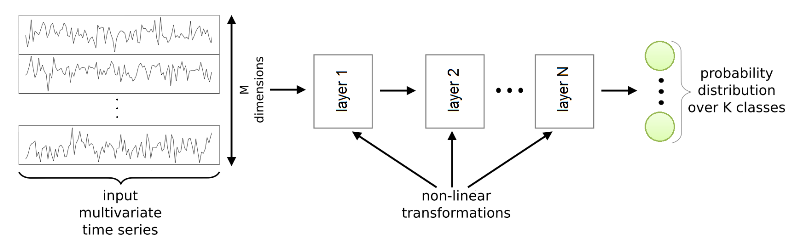
\includegraphics[width=\textwidth]{figures/project/app1.png}
    \end{minipage}
    \caption{The general Deep Learning framework for time series classification.}
    \label{fig:a1}
\end{figure}

\subsection{Convolutional Neural Networks}

Since AlexNet \cite{Krizhevsky2017ImageNetNetworks} won the imageNet competition in 2012, deep CNNs have seen a lot of successful applications in many different domains such as reaching human-level performance in image recognition problems as well as different natural language processing tasks. Motivated by the success of these CNN architectures in these various domains, researchers have started adopting them for time series analysis \cite{Gamboa2017DeepAnalysis}. 

The challenge of using this architecture is changing time series data to image data. Some papers used several techniques like Continuous Wavelet Transform (CWT) \cite{Wang2021AutomaticNetwork}, Recurrence Plots (RP) \cite{Hatami2017ClassificationNetworks}, and short-time Fourier transform (STFT) \cite{Huang2019ECGNetwork} to produce a 2D representation of time-series. Therefore, time series classification can change to a texture image recognition task.

Weng et al. in \cite{WangTimeBaseline} used a 1D convolutional operation to adapt this architecture to time series data. They tested three deep neural network architectures, MLP, FCN and Residual Network, to provide a comprehensive baseline model in time series.




\subsection{Inception Time}
Recently a deep Convolutional Neural Network called Inception Time was introduced by Fawaz et al. in \cite{IsmailFawaz2020InceptionTime:Classification}. This kind of network shows high accuracy and scalability. As shown in figure \ref{fig:a2}, the Inception Network consists of a series of Inception Modules followed by a Global Average Pooling Layer and a Fully Connected Layer (usually a Multi-Layer Perceptron). Moreover, a residual connection is added at every third inception module. Each residual block’s input is transferred via a shortcut linear connection to be added to the next block’s input, thus mitigating the vanishing gradient problem by allowing a direct flow of the gradient.

\begin{figure}[H]
    \centering
    \begin{minipage}[b]{\textwidth}
        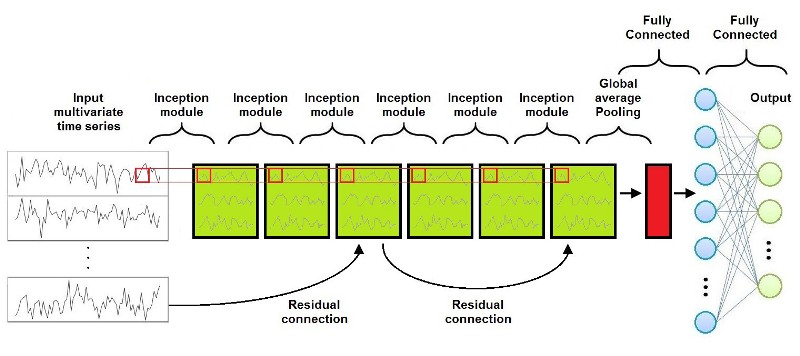
\includegraphics[width=\textwidth]{manuscript/src/figures/project/app2.jpeg}
    \end{minipage}
    \caption{Inception Network Architecture \cite{IsmailFawaz2020InceptionTime:Classification}}
    \label{fig:a2}
\end{figure}


\subsection{Echo State Networks}

Echo State Networks \cite{Bianchi2018ReservoirSeries} are a type of Recurrent Neural Network. Hence it can be useful to have a small introduction about them. Recurrent Neural Networks are networks of neuron-like nodes organized into successive layers, with an architecture similar to one of the standard Neural Networks. In fact, like in standard Neural Networks, neurons are divided into the input layer, hidden layers and output layers. Each connection between neurons has a corresponding trainable weight.  

As shown in figure \ref{fig:a3} , the architecture of an Echo State Network consists of an Input Layer, a hidden Layer called Reservoir, a Dimension Reduction Layer, a Fully Connected Layer called Readout, and an Output Layer.

In general, the main difficulty in using CNNs is that they are very dependent on the size and quality of the training data. To solve this problem, many new algorithms were recently elaborated, and among these Inception Time and Echo State Networks perform better than the others. 

Inception Time, figure \ref{fig:a2} is derived from Convolution Neural Networks and speeds up the training process using an efficient dimension reduction in the most important building block, the Inception Module. Echo State Networks are really helpful to handle chaotic time series. Hence, high accuracy and high scalability make these new architectures the perfect candidate for product development.
\begin{figure}[H]
    \centering
    \begin{minipage}[b]{\textwidth}
        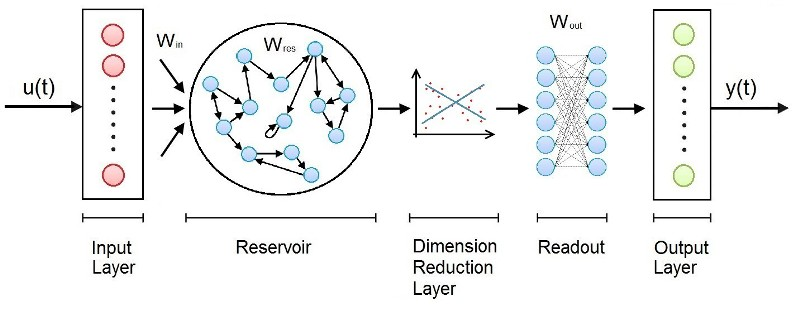
\includegraphics[width=\textwidth]{manuscript/src/figures/project/app3.jpeg}
    \end{minipage}
    \caption{Echo State Networks Architecture \cite{Bianchi2018ReservoirSeries}}
    \label{fig:a3}
\end{figure}

\end{document}